\chapter{Face Quality Assessment}
\label{chap:FQA}
The third chapter of the thesis introduces the reader to key definitions and concepts, within the field of face quality, used throughout the project. We will throw light on face image quality with examples and elaborate how face recognition systems and the two face image quality metrics behave.  

\section{What is a good image?}
\label{sec:setup}
Throughout this thesis we will mention the word quality several times. While some people already have a good understanding of what the word means, some confusion may arise. 

Within the standard image quality assessment field, the definition of quality is straight forward and is what most people think about when hearing the word. Ordinary people and people working with images will for the most part think about the image resolution as the most important characteristic that defines image quality. An excellent image of a face with this definition would have high resolution and sharp focus.   

However Mobai´s and our definition differs from the usual way image quality is defined. Our emphasis lies not with the image resolution itself, but with how well the face is visible. There are several aspects that heavily affect the quality of facial images with respect to biometric systems performance. These aspects are presented and discussed in two important papers: 
%
\begin{itemize}
    \item ISO/IEC TR 29794-5:2010: Information technology — Biometric sample quality — Part 5: Face image data \cite{ISO50912}.
    \item ICAO Doc 9303 Part 3: Specifications Common to all MRTDs \cite{ICAO1}. 
\end{itemize}
%
The quality specific aspects of facial images presented in the two standards are what defines the quality in our thesis. The different quality factors are:  

\begin{itemize}
    \item Scenery characteristics like lighting or background.
    \item Characteristics like the consistency between the skin colour on the image and the skin colour of the subject.
    \item Complete or partial face coverings.
    \begin{itemize}
        \item Glasses fully covering the eyes.
        \item Any type of head coverings.
    \end{itemize}
    \item The behaviour of the subject.
    \begin{itemize}
        \item Closed or open eyes.
        \item Closed or open mouth.
        \item Any kind of expression, e.g. smiling or neutral.
        \item Head pose, e.g. frontal or rotated in any direction.
    \end{itemize}
    \item Image properties like the size of the image or its resolution.
    \item Image appearance characteristics like the exposure or noise.
\end{itemize}

The above mentioned aspects all affect the quality of the facial image to some degree. What we consider an excellent facial image is similar to a standard passport image with the following characteristics: 
\begin{itemize}
    \item Open and visible eyes.
    \item No dark tinted glasses. 
    \item Neutral or little to none facial expression.
    \item Neutral head pose.
    \item No garments covering the face.
    \item Clean background.
    \item Neither too dark or too light.
    \item Photo taken neither too close or too far away.
\end{itemize}

The characteristics will affect the quality in a good or bad way. If all the bullet points above are true, the quality of the facial image is near perfect. An image of a half-covered or missing face will negatively affect the quality, even though the image resolution itself may be impeccable. 

\begin{figure}[h]
\centering
    \subfloat[Excellent facial image]
        {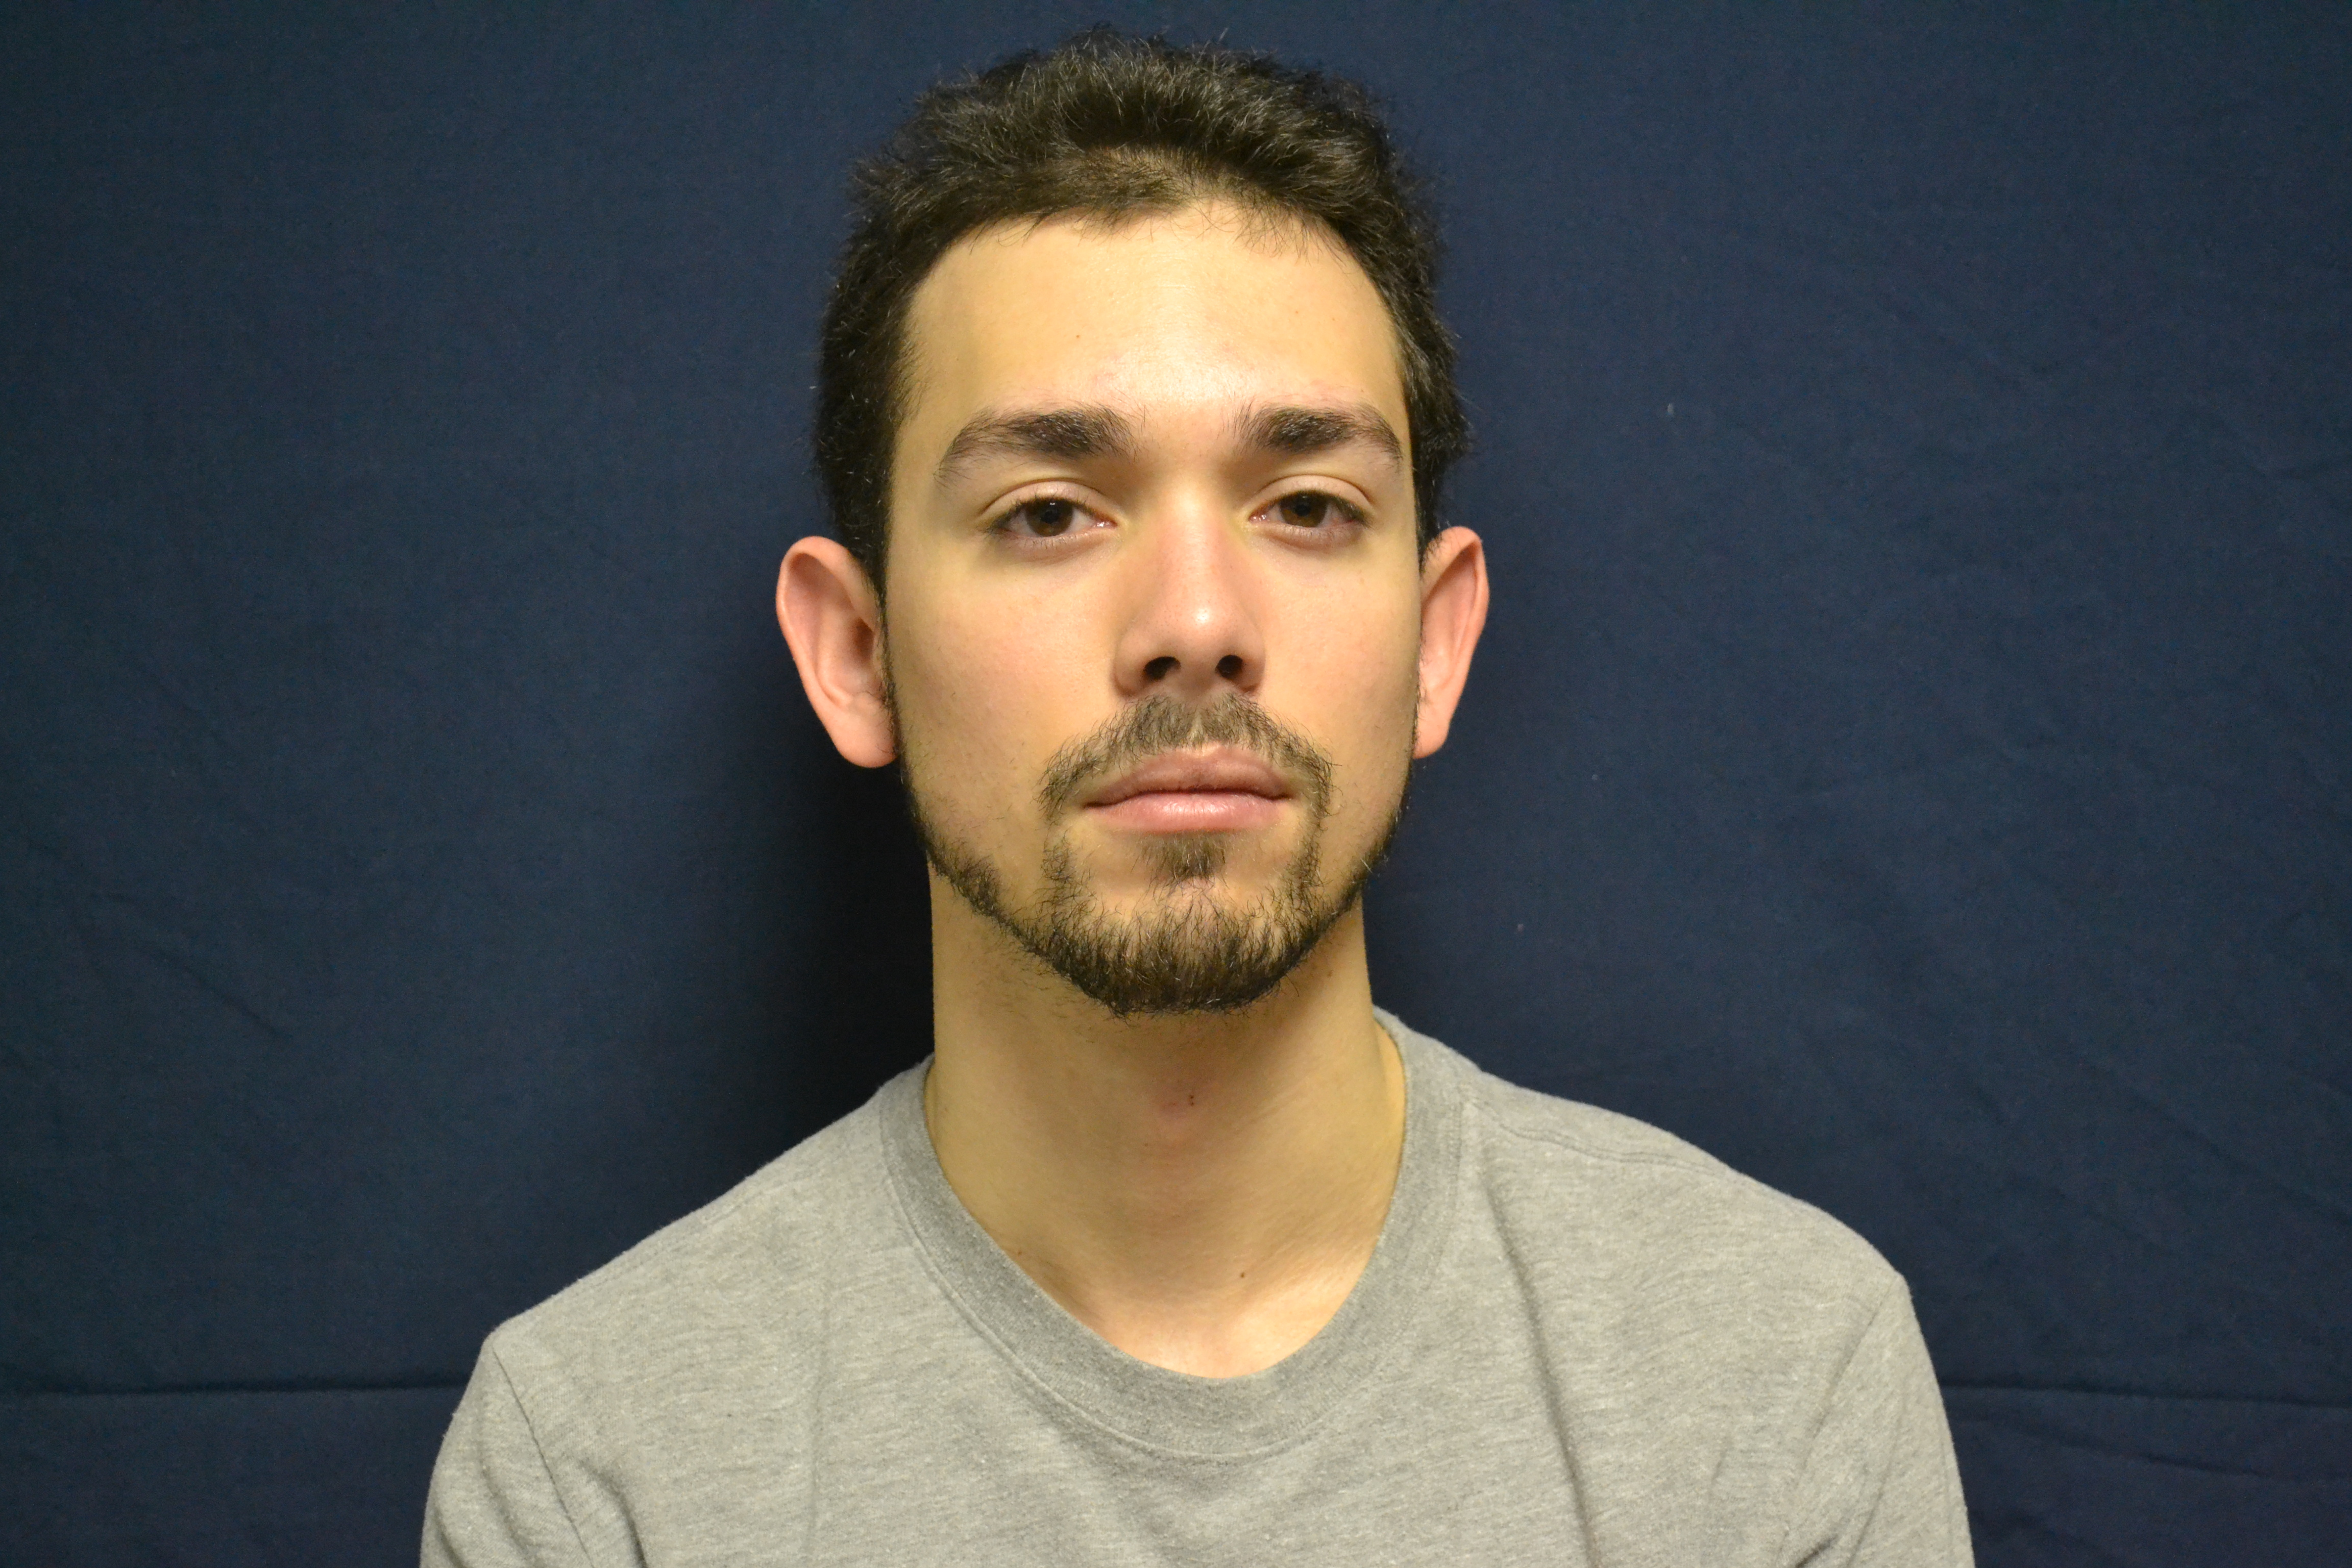
\includegraphics[scale = 0.15]{figures/ExcellentImg.jpg}
        \label{fig:excellentImg}\hspace{1.5cm}}
    \subfloat[Facial image with defects]
        {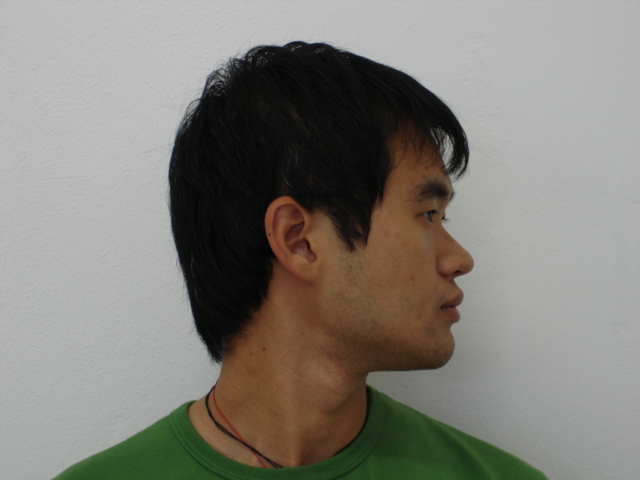
\includegraphics[scale = 0.23]{figures/FairImg.jpg}
        \label{fig:defectedImg}}
    \caption{Difference in face quality}
\end{figure}

Image \ref{fig:excellentImg} checks all bullet points in what defines an excellent image. The subjects' facial expression and head pose is neutral and the whole face is clearly visible. The second image \ref{fig:defectedImg} however does have some flaws. The main reason these two images greatly differ in quality is because of the head rotation. The head is rotated 90 degrees to the side which makes vital parts of the face far less visible. The facial image with defects does have a neutral background with good lightning and image resolution, but those aspects does not weight up against the head pose.

\begin{figure}[h]
\centering
    \subfloat[Use of face coverings]
        {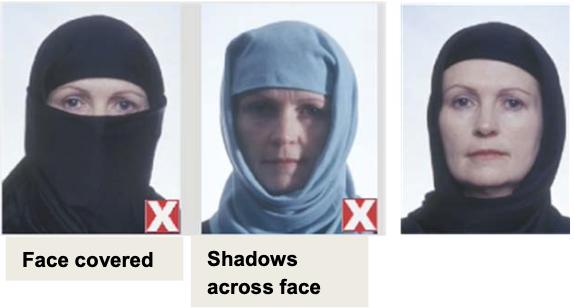
\includegraphics[scale = 0.55]{figures/FaceCovered.png}
        \label{fig:faceCovered}}
    \subfloat[Use of glasses]
        {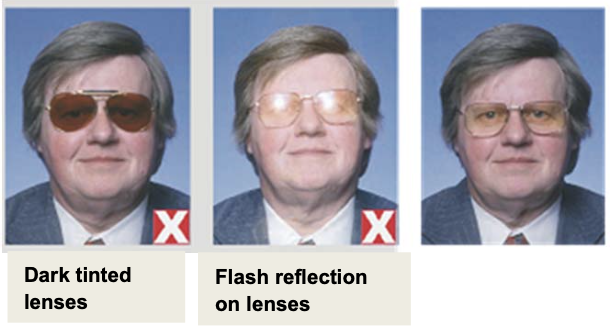
\includegraphics[scale = 0.55]{figures/SunglassesTinted.png}\hspace{1.3cm}
        \label{fig:glasses}}
        \vspace{0.5cm}
        \newline
    \subfloat[Facial expressions]
        {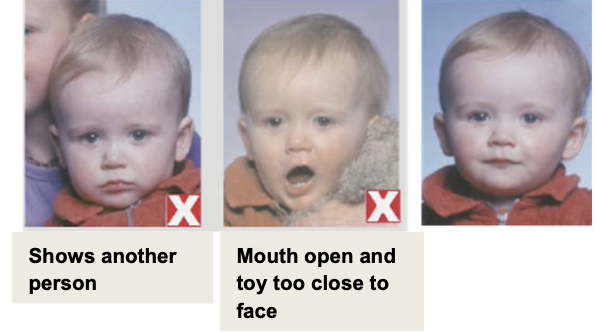
\includegraphics[scale = 0.55]{figures/BabyOpenMouth.png}
        \label{fig:babyMouth}}
    \caption{Subject lineups \cite{ICAO1}}
    \label{fig:ICAOlineup}
\end{figure}

The three image lineups in Figure \ref{fig:ICAOlineup} showcases typical flaws of facial images that negatively affect the quality. The last image of each lineup is considered to have the best quality. The flaws described varies in severity. The face image quality of the lady with her face covered would be at the bottom of the quality scale. The first two images of the man, would not affect the quality to the same degree and the quality of the first two images of the kid, would affect the quality even less. 
\newpage

\section{Face image quality metrics} 
With the inclusion of authentication to applications, face recognition (FR) systems are being utilized more than ever. These FR systems are reliant on a reference image, which is pre-captured, to compare with a probe image for identity recognition. 

\begin{figure}[h]
    \centering
    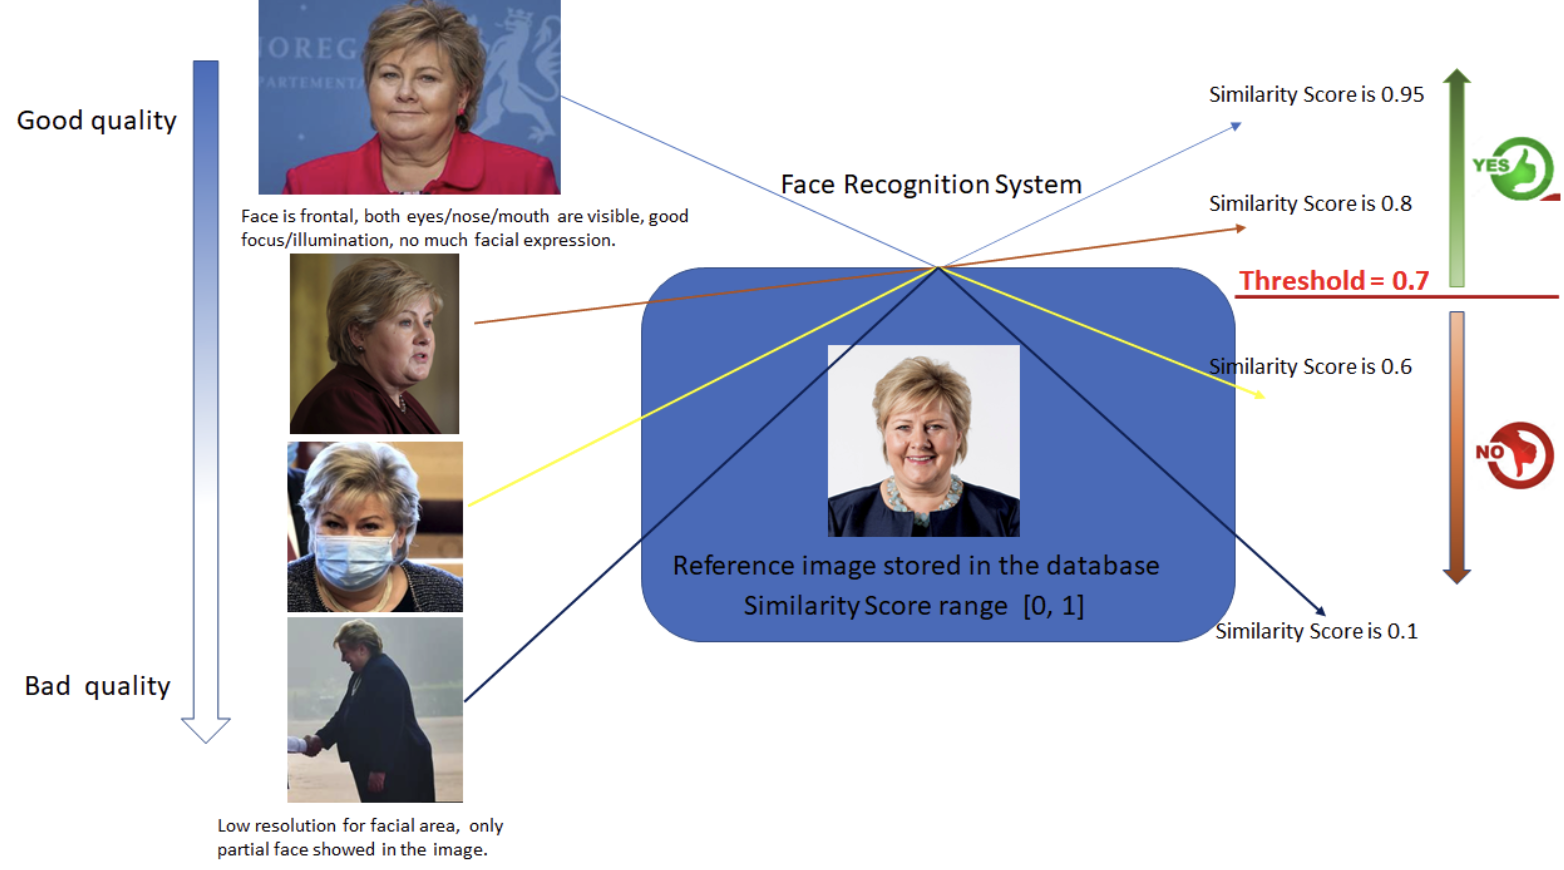
\includegraphics[scale = 0.45]{figures/Erna.png}
    \caption{Face recognition system}
    \label{fig:erna}
\end{figure}

Figure \ref{fig:erna} visualizes how FR systems work. The probe images´s qualities, on the left side of the figure, are assessed and then used to compare with a reference image. The reference image is of the best quality. A similarity score between the two images is calculated, and in this case the similarity score is between zero and one. FR systems have a set threshold where probe images are rejected if the similarity score is too low. 

As mentioned in Section \ref{section:background}, Mobai is currently using such a FR system. The performance of the system is affected by the quality of the probe images. If the probe images are of bad quality, the overall performance of the system will be degraded. This is where the FIQMs are relevant. The metrics can be used to reject and filter images of low quality and therefore only allow images of high quality to be used in the FR system. 
\newpage

\begin{figure}[h]
    \centering
    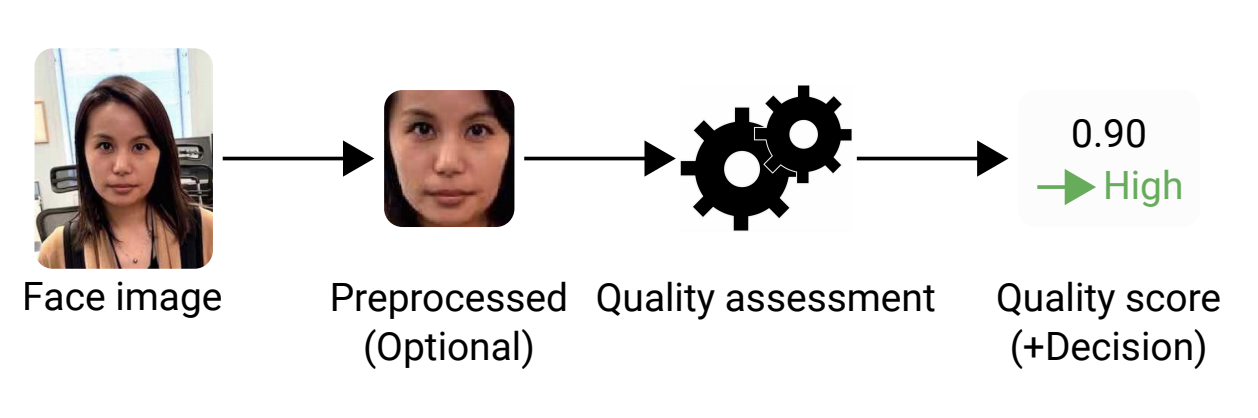
\includegraphics[scale = 0.45]{figures/FIQM.png}
    \caption{Typical FIQM process \cite{FaceImageQualityAssessment}}
    \label{fig:fiqm}
\end{figure}

FIQMs are automated algorithms that take images as input, does some calculations, and return a quality estimate score. FIQMs can be based on different quality factors, such as subject-camera distance, inter-eye distance, pose, lightning and facial coverings. 

FIQMs can be divided into three approaches in regards to a reference image. It is important to understand that these reference images have nothing to do with the reference images mentioned in the FR system. These reference images are only used for the FIQMs. The three approaches are: 

\begin{itemize}
    \item Full-reference.
    \item Reduced-reference.
    \item No-reference. 
\end{itemize}

The names of the approaches are telling of what to expect. The full-reference approach compares the input image against a known reference image of good quality. The reduced-reference approach is similar to the above mentioned approach, however only some of the information in the reference image is used. At last, the no-reference approach does not require a reference image to calculate a score. 

Mobai chose the FIQMs used in our application. The reason for choosing these specific metrics was their differences in terms of evaluating images of faces. The two FIQMs are both no-reference approaches which will be used to assist and provide feedback when an image is acquired for FR system enrollment. 


\subsection{ISO metrics}
ISO metrics is a non-referenced face image quality metric. The metric is implemented based on ISO/IEC TR 29794-5:2010 Information technology — Biometric sample quality — Part 5: Face image data. Different factors that affects the face image quality are considered in the implementation. 

\subsubsection*{Filter by eye distance}
The ISO metrics calculates the inter-eye distance on facial images passed in the metric. If this value is below a certain criteria, the metric will filter out these type of images. The inter-eye distance is related to subject camera distance, because it indicates that the subject could be too close to or too far from the camera lens. 

\subsubsection*{Image properties and characteristics}
\label{subsubsection:image properties and characteristics}
ISO metrics takes all image properties and characteristics described in the ISO paper into account when evaluating facial images. It calculates the image's sharpness, contrast, blur, brightness, exposure, pose symmetry, light symmetry and illumination symmetry. These factors are stored in an array for each facial image. 

\subsubsection*{Predicting the quality score}
To be able to calculate quality scores on the facial images, train data are needed. The metric uses random forest regression \cite{RandomForestRegressor} with 214 trees, 22 nodes of depth and the dataset is used to build each tree. Quality scores of the facial images are computed by predicting the image properties array described in \ref{subsubsection:image properties and characteristics}. 

\subsection{FaceQnet}
FaceQnet \cite{FaceQnet} is an open source, no-reference face quality assessment tool based on deep learning. FaceQnet has two versions implemented, FaceQnet v0 and FaceQnet v1. The newest, FaceQnet v1, was used for this project. Its quality measures is closely related to the ICAO \cite{ICAO2} standard that provides strict guidelines for capturing images. Factors such as illumination, pose, resolution and focus are essential in regards to the quality.

\subsubsection*{Face cropping}
In figure \ref{fig:fiqm} the second step, data preprocessing, is optional. That step is key in the implementation of FaceQnet. Generally data preprocessing removes unnecessary data, which directly improves the quality of machine learning algorithms. 

The background of images will affect the quality score which provides us with biased results. One way to avoid feature extraction from the background, is to crop the input images to only match the face before using FIQMs. FaceQnet uses multitask cascaded convolutional networks (MTCNN) to detect and extract the coordinates of the faces. Thereafter the facial image is cropped to an $224 \times 224 \times 3$ image according to the bounding box and used as the input image to the FIQM. 

\subsubsection*{Training data}
FaceQnet uses the VGGFace2 \cite{VGGFace2} database to create a pretrained model to make its quality prediction. The VGGFace2 database is quite large with over 3.31 million images of 9131 subjects which is why FaceQnet only uses a subset of 300 subjects. The algorithm will first generate ground truth quality measures which is created by labeling the 300 subjects in the training database. The ground truth quality measures will then train the deep regression model in order to generate quality scores. After the model is trained, it is ready to receive the probe images. The data provided to the FIQM is loaded and split into test data (X\_test and y\_test) which are used to get a quality estimate. 

